%=====================================================
%====== If you are new to LaTeX, this website ========
%======     will be your new best friend:     ========
%======   http://en.wikibooks.org/wiki/LaTeX  ========
%======   Template created by Jonathan Blair  ========
%=====================================================



%=====================================================
%============ Controls ===============================
%=====================================================

%\documentclass[12pt,letterpaper,onecolumn]{article}
\documentclass[11pt,letterpaper,onecolumn]{article}
%\documentclass[10pt,letterpaper,onecolumn]{article}  % not recommended
%\documentclass[12pt,letterpaper,twocolumn]{article}
%\documentclass[11pt,letterpaper,twocolumn]{article}
%\documentclass[10pt,letterpaper,twocolumn]{article}


\usepackage{amsmath}
\usepackage{graphicx}
\usepackage{url}
\usepackage{textgreek}
\usepackage{float}
\usepackage{booktabs}
%\graphicspath{{path-to-folder-containing-necessary-graphics}{other folder as necessary}}


%=====================================================
%============ \begin{document} =======================
%=====================================================

\begin{document}

%=====================================================
%============ Title ==================================
%=====================================================

\title{\bf Observing the Behavior of RC Circuits}
%\title{\Large\bf Larger, Bolded Title}

%=====================================================
%============ Author =================================
%=====================================================
\author{
 Jairo Portillo \\*
  \\*
 PHY 338K Electronic Techniques \\*
 Department of Physics \\*
 The University of Texas at Austin \\*
 Austin, TX 78712, USA
}
\date{February 3, 2016}

%\address{The University of Texas, Austin, Texas, 78712}

\maketitle

%=====================================================
%============ Abstract ===============================
%=====================================================

\begin{abstract}

In this lab, we will observe and study the behavior of RC circuits. We will observe the time domain and frequency domain of high pass and low pass filters with a resistor and capacitor. We observed that a low pass filter blocks out frequencies higher than the cut off frequency of 5.38 kHz and high pass did the exact opposite.
\end{abstract}

%=====================================================
%============ Body of the article ==========================
%=====================================================

%=====================================================
%============ Section ==================================
%=====================================================

\section{Preparation}

In order to prepare for this lab, we had to review the response of RC circuits and derive the transfer function for each circuit and the step function transient response. In order to find the step function we must use Kirchhoff laws and fund that an equivalent current flows through the circuits which lead us to conclude that 
$$I=C\frac{dV}{dt}= \frac{V_{in}-V_{out}}{R}$$
With this we find that
$$V_{out}=V_0(1-e^{\frac{-t}{RC}})$$
where R is the resistance and C is the capacitance. $RC$ is equivilant to the period of the system. In order to find the transfer function $T(\omega)$ we simply use the relation 
$$T(\omega) = \frac{V_{out}}{V_{in}}=\frac{Z_{out}}{Z_{in}+Z_{out}}$$
where $Z_{out}$ is the impedance for the output voltage and $V_{in}$ is the impedance for the input voltage both varying depending on the filter. For low pass is becomes 
$$T(\omega)=\frac{Z_C}{Z_C+R}=\frac{\frac{1}{j\omega C}}{R+\frac{1}{j\omega C}}=\frac{1}{\sqrt{1+R^2C^2\omega^2}}$$
and for high pass it would be
$$T(\omega)=\frac{R}{Z_C+R}=\frac{R}{R+\frac{1}{j\omega C}}=\frac{R\omega C}{\sqrt{1+R^2C^2\omega^2}}$$
where $Z_C$ is the impedance of the capacitor, $\omega$ is the frequency, and $j$ is $\sqrt{-1}$.
The behavior of the low pass RC circuit can bee seen with high frequencies as the impedance of the capacitor become much smaller than that of the resistor or $\frac{1}{\omega C}<<R$ therefore making the resistors potential much greater $V_R >> V_C$. Since $V_{in} = V_R + V_C$ and with the initial condition previously mentioned we can conclude that $V_{in} \approx V_R$ as $V_C$ is insignificant compared to $V_R$, with this we know that the current is $\frac{V_{in}}{R}$. With this information and that $V_{out} \approx V_C$ we can see that 
$$V_{out} = \frac{Q}{C}=\frac{1}{C}\int^t_0 I_{in}\,dt=\frac{1}{RC}\int^t_0 V_{in}\,dt$$
With this we can see that the output voltage increases proportionally to the frequency times the sum of the input voltage over time. With the high pass filter, we use the conditions 

$$\frac{1}{\omega C} >> R \text{; } V_R<<V_C \text{; } V_C \approx V_{in} \text{; and }$$
$$ V_{in} = \frac{1}{C}\int^t_0 I_{in}\,dt \Longrightarrow \text{ } I_{in}=C\frac{d}{dt}V_{in}$$

we find that the output voltage is
$$V_{out} \approx V_R = RC\frac{d}{dt}V_{in}$$
where we can see that the output voltage is proportional to the period times the rate of change of the input voltage.

\section{Labwork}


\subsection{Apparatus}

Our apparatus was  a signal generator connected with a Tee and BNC to the oscilloscope in channel 1. The Tee allowed grabber connections to be attached for the input of the circuit. The output of the circuit was grabber connections to a BNC into channel 2 of the oscilloscope. We used a 74 $\Omega$ resistor and a 0.399 $\mu F$ capacitor. We set up the resistor and the capacitor on a bread board that held the circuit. Switching between high pass and low pass was simply in a matter of switching where in input and out put were with respect to the circuit on the bread board.   


%=====================================================
%============ Importing pictures  ==========================
%=====================================================

% !! To be imported, all graphics must be converted !!
% !!    to encapsulated postscript (.eps format)    !!
% !!  The GNU Image Manipulation Program (GIMP) is  !!
% !!          capable of this conversion.           !!



\subsection{Data Collection}

A majority of our data came from the oscilloscope as it had features that measured the voltage, frequency, and phase shifts in the signals. In order to collect data we did what was recommended and took two point per decade until we saw a significant change. When that change occurred, we returned to that frequency range and took a few more points. We took data from Hz to kHz. 

\begin{figure}[H]
    \centering
    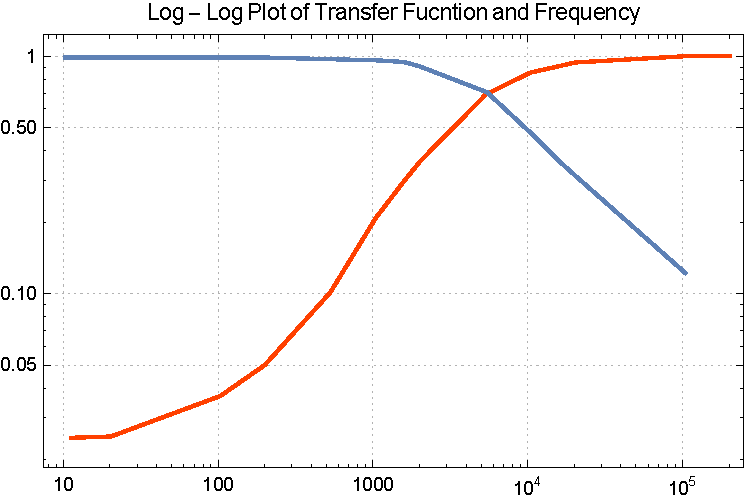
\includegraphics[scale = .8]{HighLowpassLogLog.pdf}
    \caption{Our Log-Log Plot. Y axis is $T(\omega)$ in the log scale and the X axis is frequency in the log scale. The Blue plot is the data from the Low pass filter. The Red plot is the data from the high pass filter.}
    \label{fig:loglog}
\end{figure}

We can see that the filter behaved just as expected where the low pass filter attenuates high frequencies and the high pass filter attenuates low frequency signals. From the graph we can see that the cut off frequency is at 5.5 kHz, which is near our calculated cut off frequency of 5.39 kHz.

\begin{figure}[H]
    \centering
    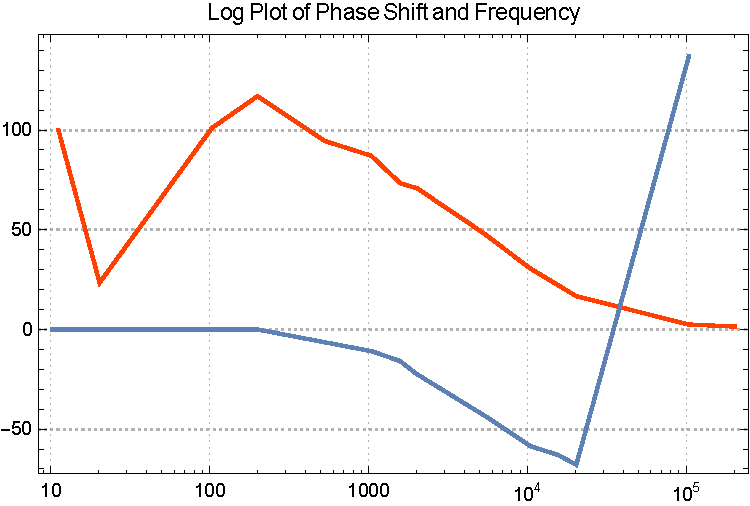
\includegraphics[scale = .8]{PhaseShift.pdf}
    \caption{Our Log Plot. Y axis is the phase shift in the log scale and the X axis is frequency. The Blue plot is the data from the Low pass filter. The Red plot is the data from the high pass filter.}
    \label{fig:log}
\end{figure}

Our phase plot does not follow what is expected thus making it difficult to draw conclusions. However, there is one conclusion that can be seen and that is that when the signal begins to attenuate a phase shift begins to appear. When the transfer function is 1 then the phase shift is 0.

\begin{figure} [H]
    \centering
    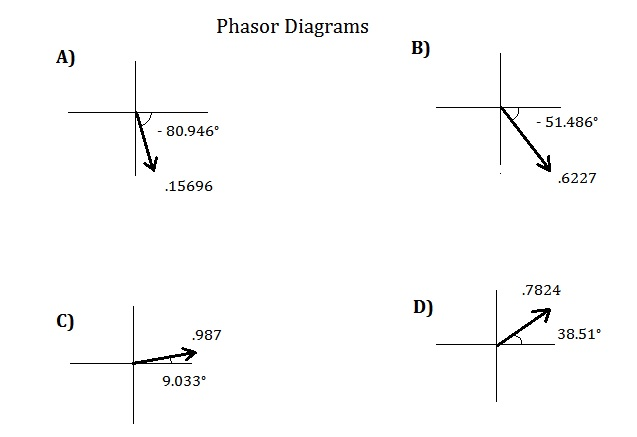
\includegraphics[scale = .8]{PhasorDiagram.jpg}
    \caption{Phasor Diagrams. A is for low pass at $f_c$, B is for low pass at $\frac{f_c}{5}$, C is for high pass at $f_c$, and D is for high pass at $\frac{f_c}{5}$. $f_c$ is the cut off frequency. }
    \label{fig:phasor}
\end{figure}

From the phasor diagram, it can be seen that as frequency decreases for a low pass filter the angle increases, while for high pass filters as the frequency decreases the angle of the phasor increases. This follows the pattern of Figure \ref{fig:log} as we can see that for the low pass filter as the frequency decreases the phase shift continues to increase to zero. Meanwhile for the high pass as the frequency increases, the phase aproaches 0. 

\begin{figure}[H]
    \centering
    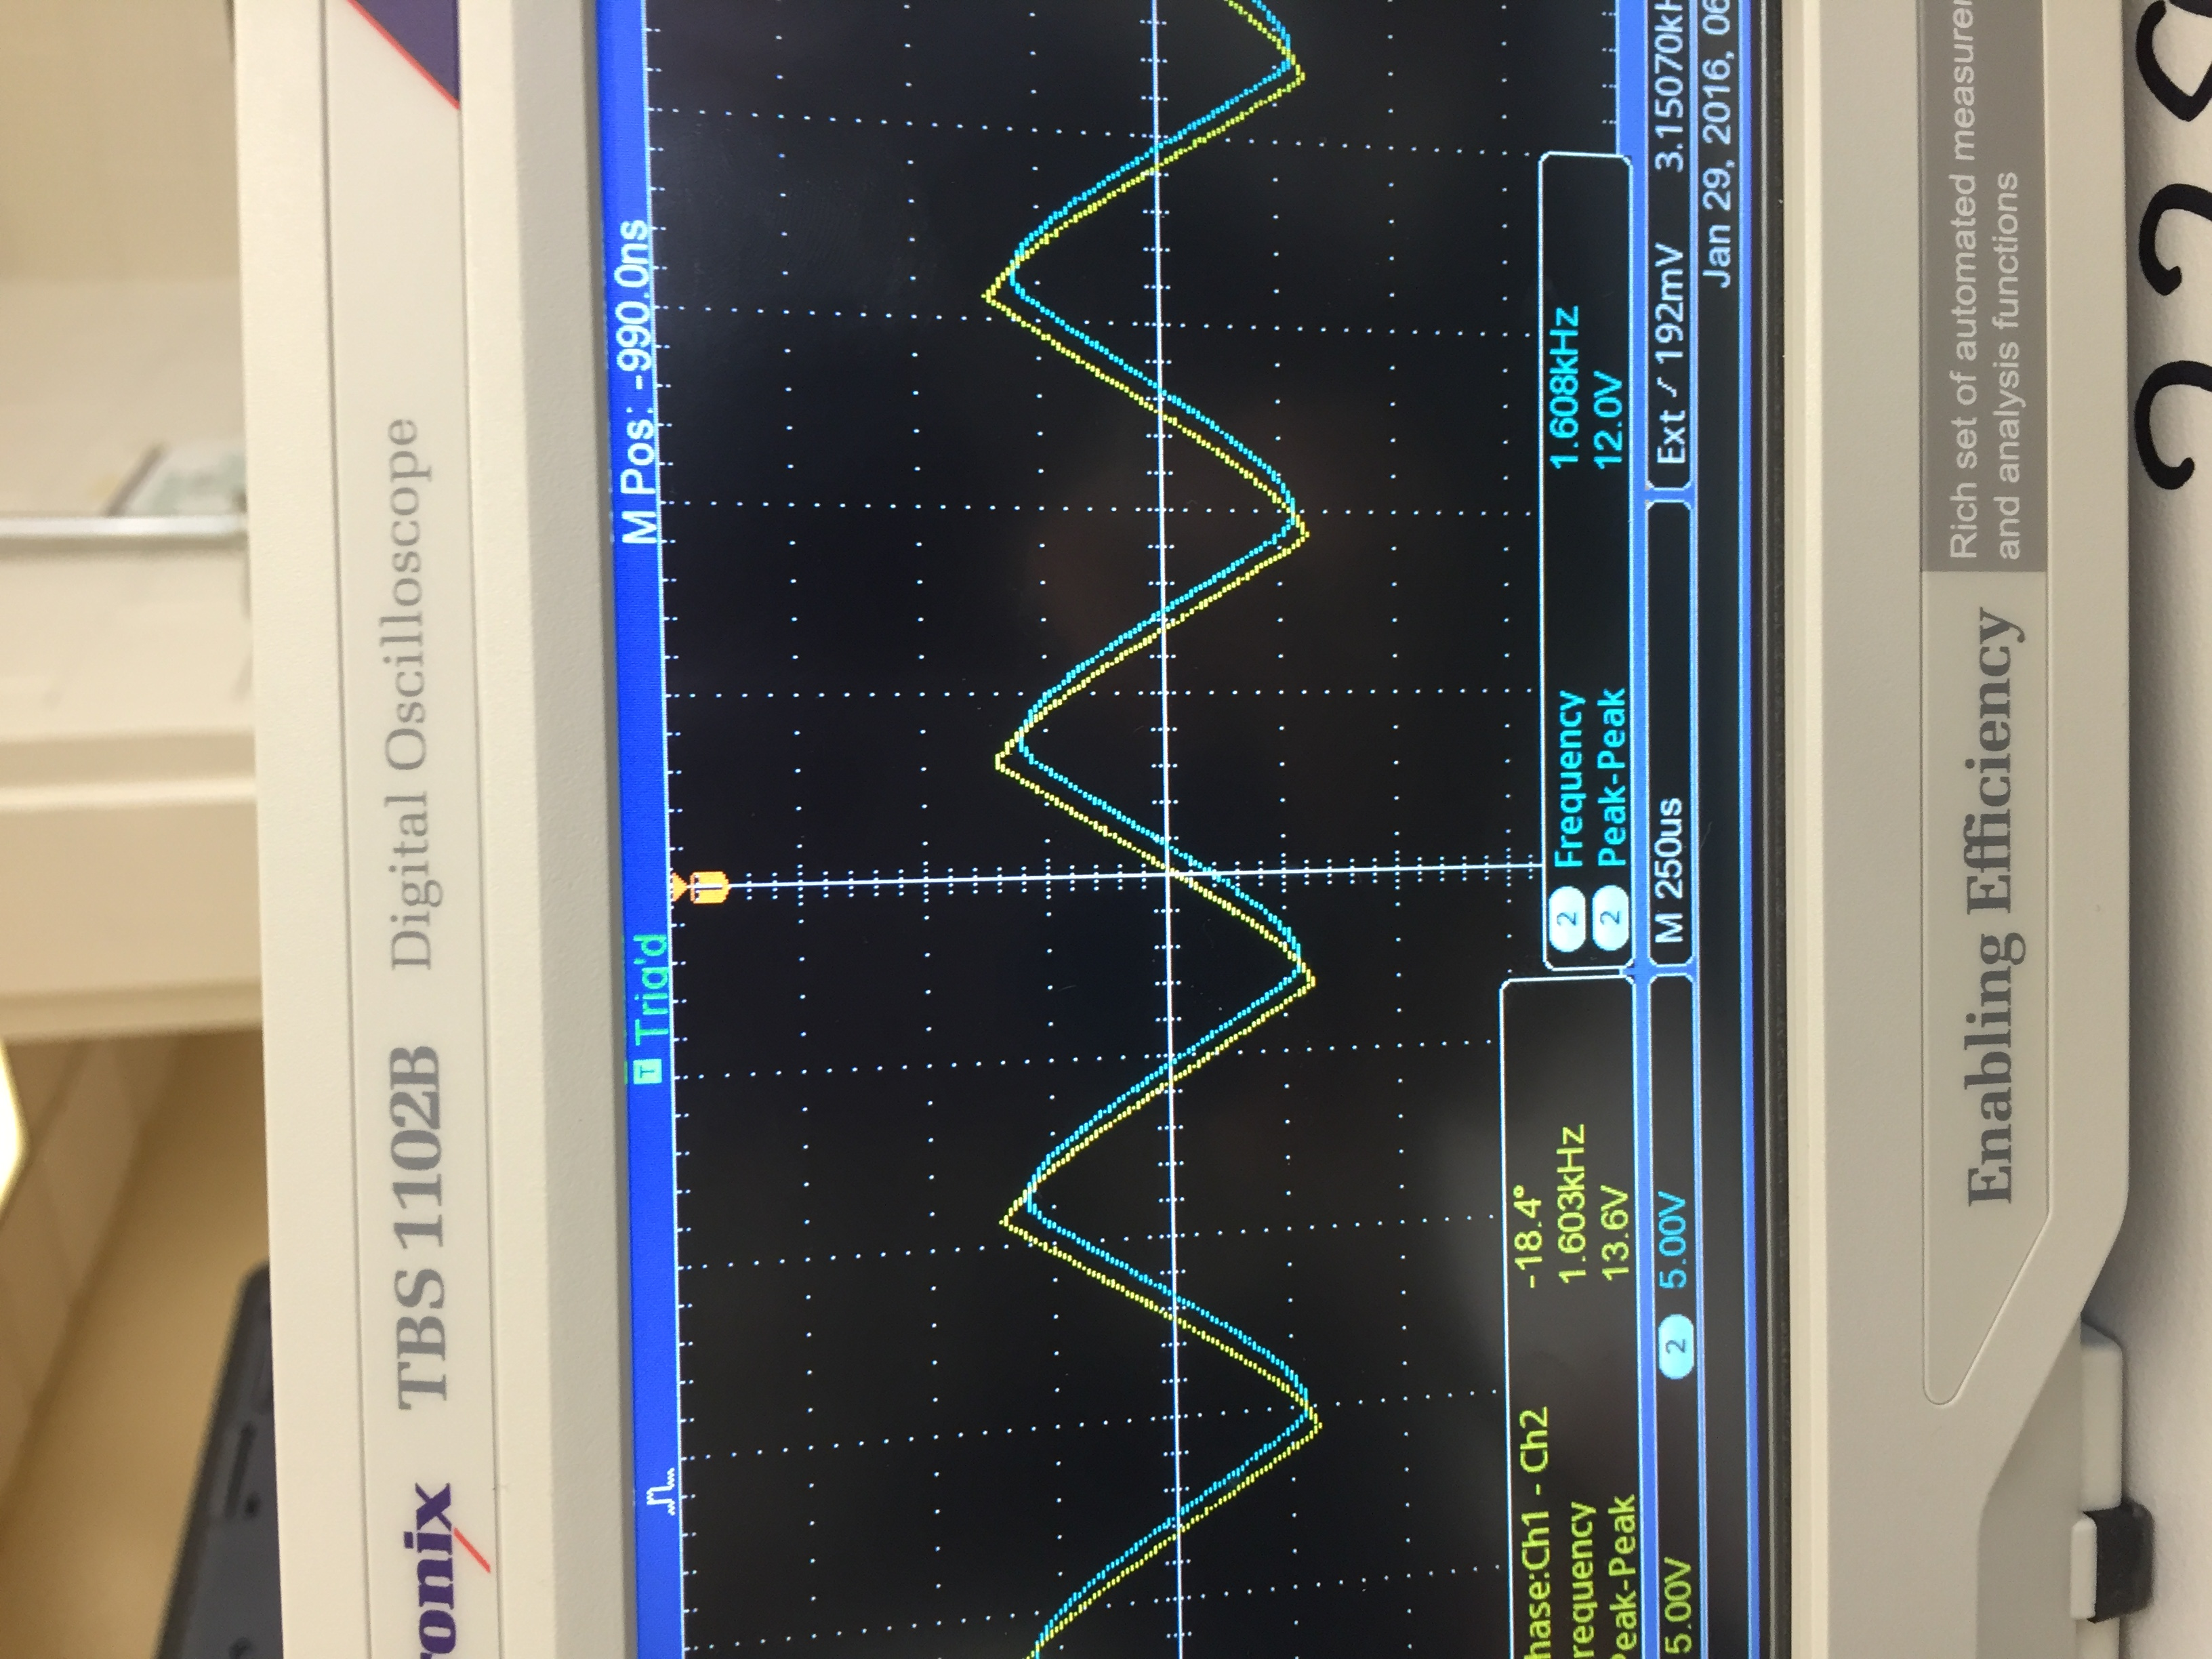
\includegraphics[scale = .1,angle = 270]{image4.JPG}
    \caption{Triangle wave going through a low pass filter. The yellow wave is the input while the blue wave is the output.}
    \label{fig:TriL}
\end{figure}

In Figure \ref{fig:TriL}, demonstrates the output of the oscilloscope when a triangle wave is passed through the low pass RC circuit. We can observe that the output is a sine wave which is the result of integration of the triangle wave. This allows the conclusion that the low pass RC circuit behaves as an integrator as shown earlier. They same effect can be seen with a square wave where the output is a skewed square wave regardless of the frequency.   

\begin{figure}[H]
    \centering
    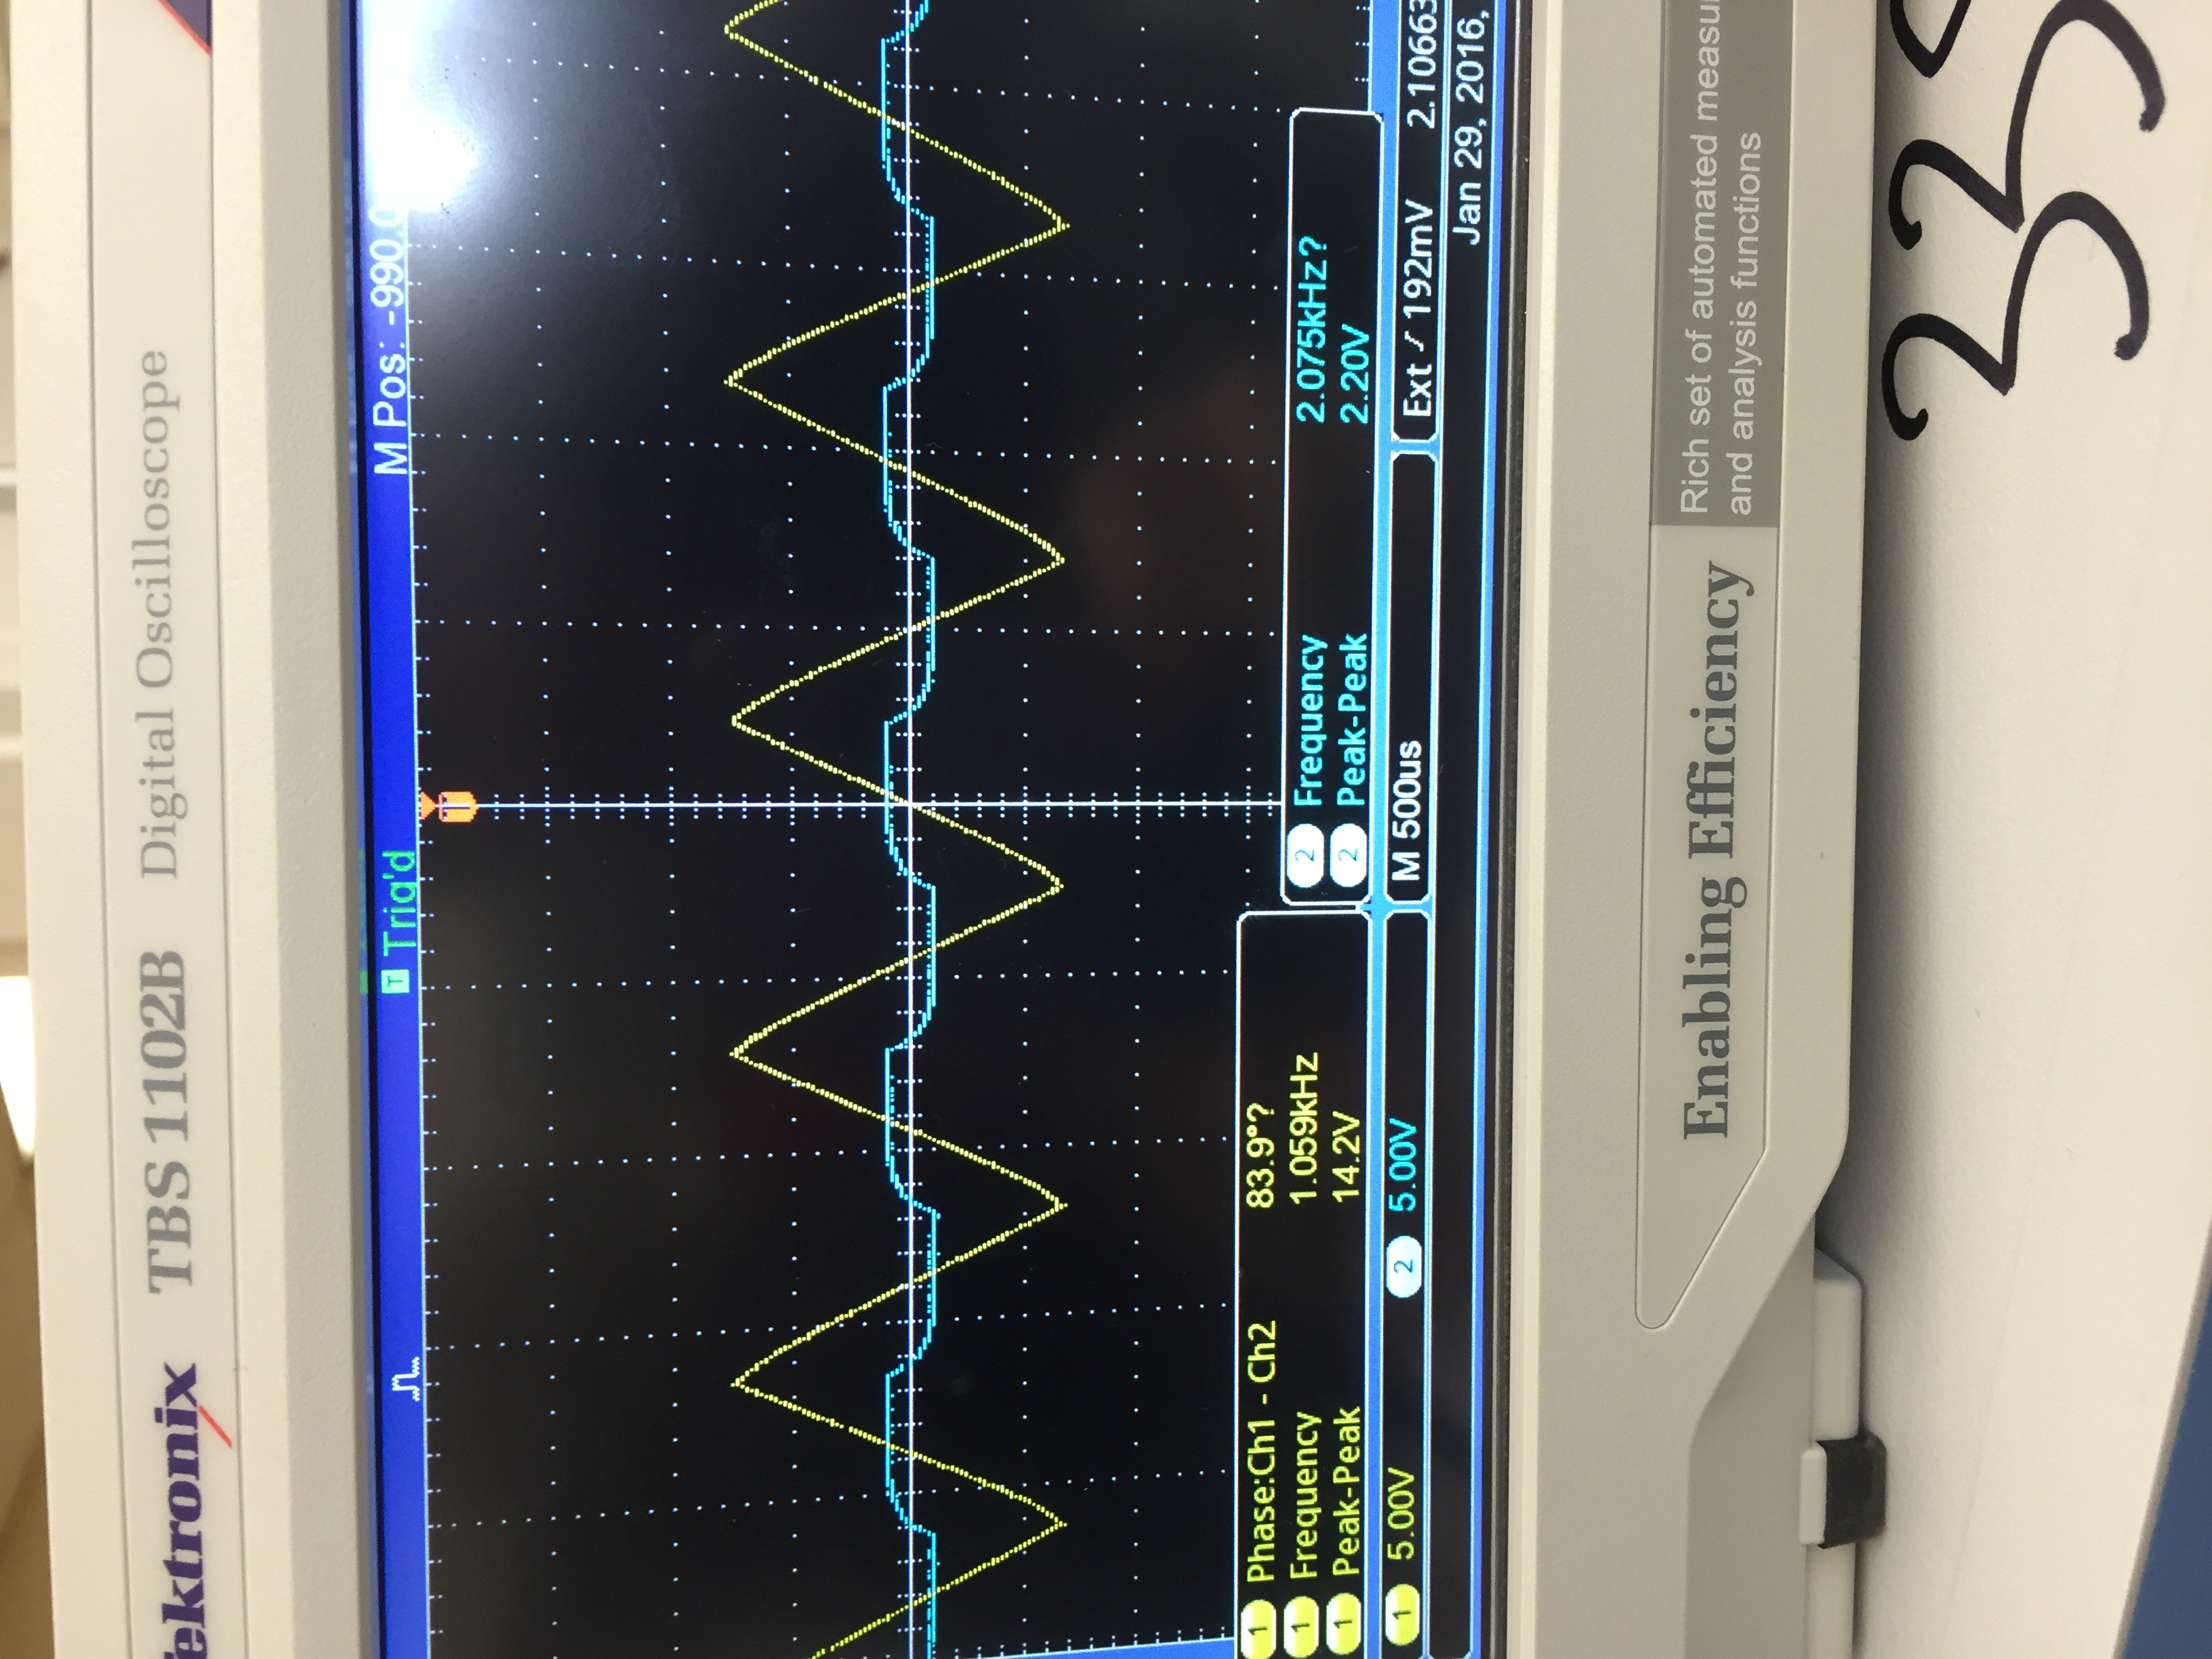
\includegraphics[scale = .1,angle = 270]{image1.JPG}
    \caption{Triangle wave going through a high pass filter. The yellow wave is the input while the blue wave is the output.}
    \label{fig:TriH}
\end{figure}

In Figure \ref{fig:TriH}, demonstrates the output of the oscilloscope when a triangle wave is passed through the high pass RC circuit. We can observe that the output is a square wave which is the result of the derivative of the triangle wave. This allows the conclusion that the low pass RC circuit behaves as a differentiator as shown earlier. The same effect can be seen in a square wave in which the output has decaying peaks for the positive square peak and increasing log peaks for negative peaks. These results are the same regardless of the input frequency.   

\section{Summary and conclusions}

We were able to observe the behavior of two types of RC circuits. From our data, we can conclude that a low pass filter prevents high frequencies from passing through and that it behaves as an integrator to the input function. We can also conclude that a high pass filter prevents low frequencies from passing through and it acts as a differentiator to the input function. It is also noted that as frequency decreases that the phase difference increases. We also found based on our circuit with a resistor of 74 $\Omega$ and a capacito 0.399 $\mu F$ that our cut off frequency was 5.5 kHz which was $2\%$ from our expected value of 5.39 kHz. 


%=====================================================
%============ Bibliography  ==============================
%=====================================================



%=====================================================
%============ End ====================================
%=====================================================

\end{document}

%=====================================================
%============ End ====================================
%=====================================================
